
\section{System}

In this section, we introduce the main components of the system. Our system is built with a pipeline architecture in mind giving it the advantage to run each section separately to allow stream processing without blocking the data flow of components (Figure~\ref{fig:system}). The three logical components include sections on \textit{Model} for entity resolution purposes, \textit{Wiki Citation} to annotate cite-worthy documents, \textit{Slot Filling} to generate the actual slot values.


To walk you through the steps we take, assume we only care about on single WP entity, the first step is to extract aliases of the entity. We use several approaches to get as many viable aliases as possible. Then we look into the stream of content that is being generated on the internet, apply two levels of filtering to finally end up with the documents are central to that entity. To extract the relevnat slot values we perform pattern matching in each sentence or coreferent sentence to see if we can find a match. As a match is found from the content of the sentence to the patterns that we have generated regarding slot name, the associated slot value is extracted as a final result.

%\ceg{Discuss current system first. If you want to keep the decisions points that led to the current architecture, make it a subsection.}

\begin{figure}
\hspace{-10mm}
  \centering
%  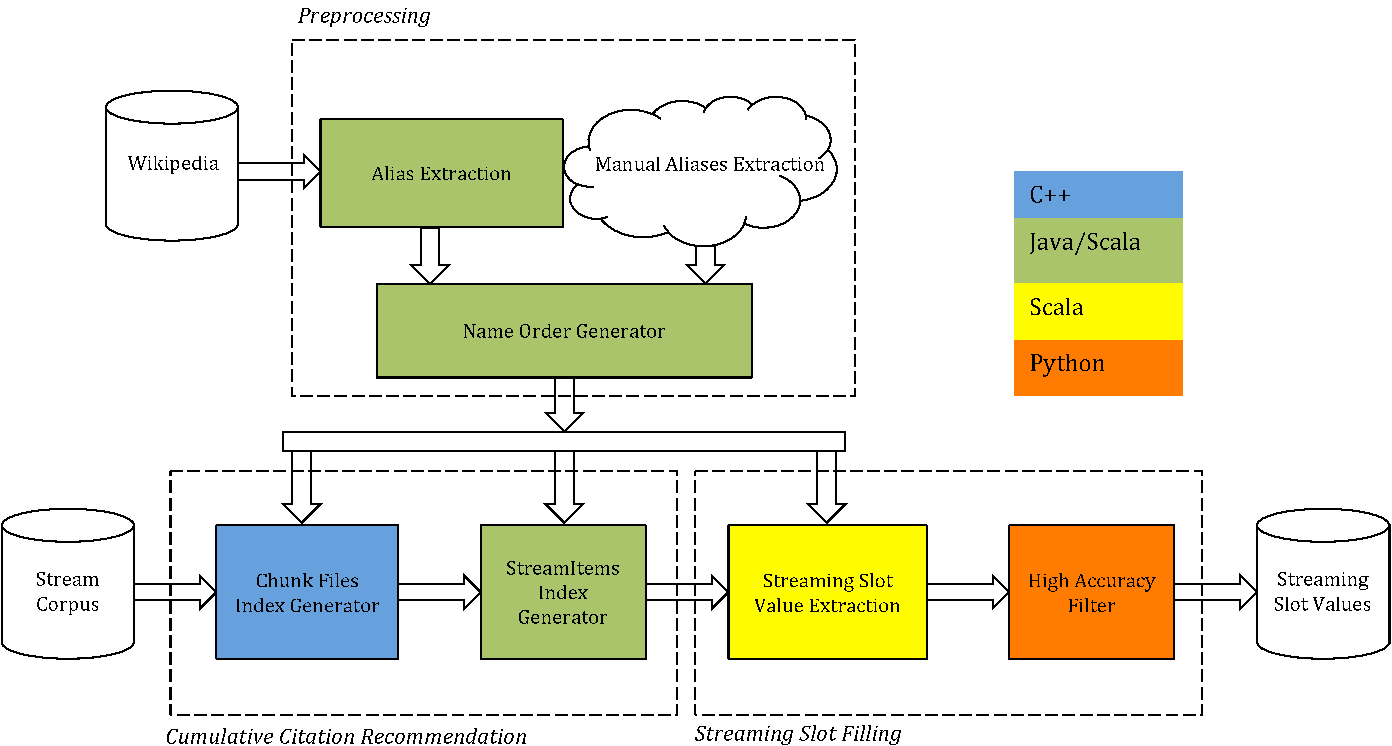
\includegraphics[width=6in]{./images/sdl-eps-converted-to.pdf}
  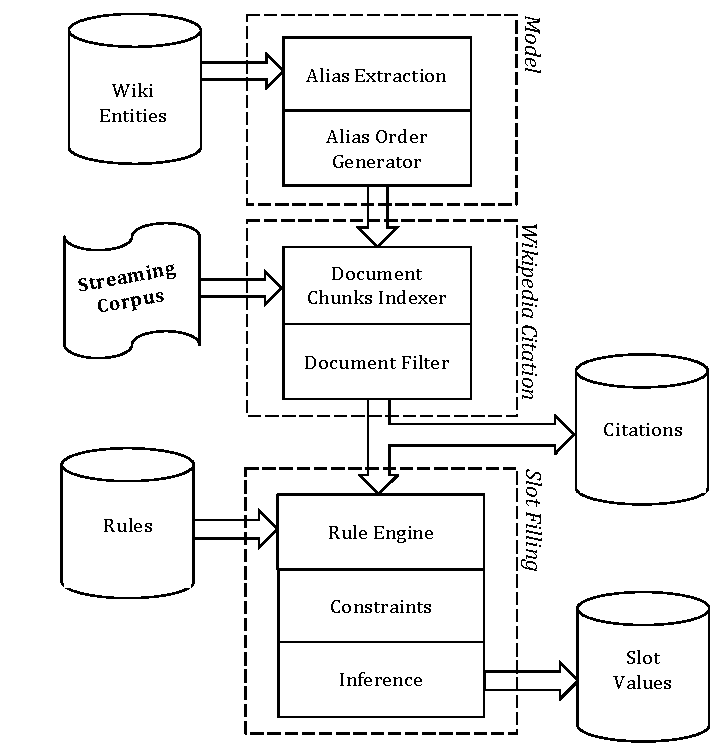
\includegraphics[width=8.5cm]{./images/System_Diagram_with_model_Vertical-crop.pdf}
% http://convert.neevia.com/pdfconvert/
  \vspace*{-.1in} 
  \caption{System Architecture.
  Components are logical groups noted with dotted boxes.}
  \label{fig:system}
  \vspace*{-.2in}
\end{figure}



\subsection{Model}

We use Wikipedia API to get these aliases automatically. This is done by retrieving backlink references (redirects of a wiki entity), e.g. William Henry Gates is an alias for Bill Gates in WP as a backlink reference. Unfortunately this is not good enough and to enhance recall we need more aliases. To have better use of a wiki page we parse HTML DOM of the page, then use regular expressions to extract the bold phrases of the first paragraph as alias of the actual entity. Based on our observation this is a very accurate heuristic and provides us with lots of famous aliases of the entities. As an example of when this might not wirk, is that there might be occasions that some other topic is written in bold typesetting in the first paraph apart from the entity aliases itself but these are very rare.

Once aliases are available we pass them through rules of generating proper name orders which will produce various forms of writing a name. As a basic example Bill Gates can be written as Gates, Bill also. This will allow the system to capture various notation forms of aliases. We refer to this part as \textit{Alias Order Generator}.

\subsection{Wikipedia Citation}
The main goal of CCR is to have an aggregate list of documents that are worthy of being cited in a Wikipedia page. We perform exact string matching and treat all the documents that mention an entity equally likely to be citable. One of the reasons for this is that in former TREC KBA reports \cite{JFrank12} there were observations of how non-mentioning documents have a low chance of being citable in Wikipedia. So we take on that and ignore non-citing documents. 

Our pipeline of processing the corpus consists of a two layer indexing system referred to as \textit{Document Chunks Indexer} and \textit{Document Filter}. Document chunks Indexer will generate indexes of the chunk files that contain a mention of any of the desired entities. Document Filter on the other hand will index documents that contain a mention of a given entity respectively. This two level indexing will eliminate the need to process each and every chunk file/document for every entity. The reason for splitting this task into two steps is that not all chunk files contain any mention of the entities and we want to get rid of them as soon as possible. Document Chunks Indexer which discards non-mentioning chunk files and will stop further processing a chunk file as soon as it finds a mention there. Each chunk file can contain up to thousands of documents which can be so time consuming if we were to process them in our Java base code. Processing StreamItems on the other hand is done in Java with ideas in mind for later on extensibility by adding other Java libraries.


% Note: Describe the algorithms of each phase
% Talk in abstract terms not implementation.
% Use formal representations (Math, SQL etc)


%\ceg{This section should be structured as follows:
%1: Introduce CCR (Motivation, Expectations)
%2: Our high level approach
%3: Discussion of our design (Like already discussed)
%}


\subsection{Slot Filling}
%\ceg{See the previous note.}
The purpose of SSF is to extract proper values for relations of interest, which can be found in Table~\ref{table:slotNameOntology}.  In Figure~\ref{fig:system} we refer to this as \textit{Slot Filling}. 

Slot filling is done by pattern matching documents with manually produced patterns for slots of interest. The way we do this is by observing a sentence that has a mention of the entity or one of its coreferences. An anchor word in the sentence related to the slot name is located and we match either left or right of the anchor word for potential slot values. 


\begin{figure}
\centering
%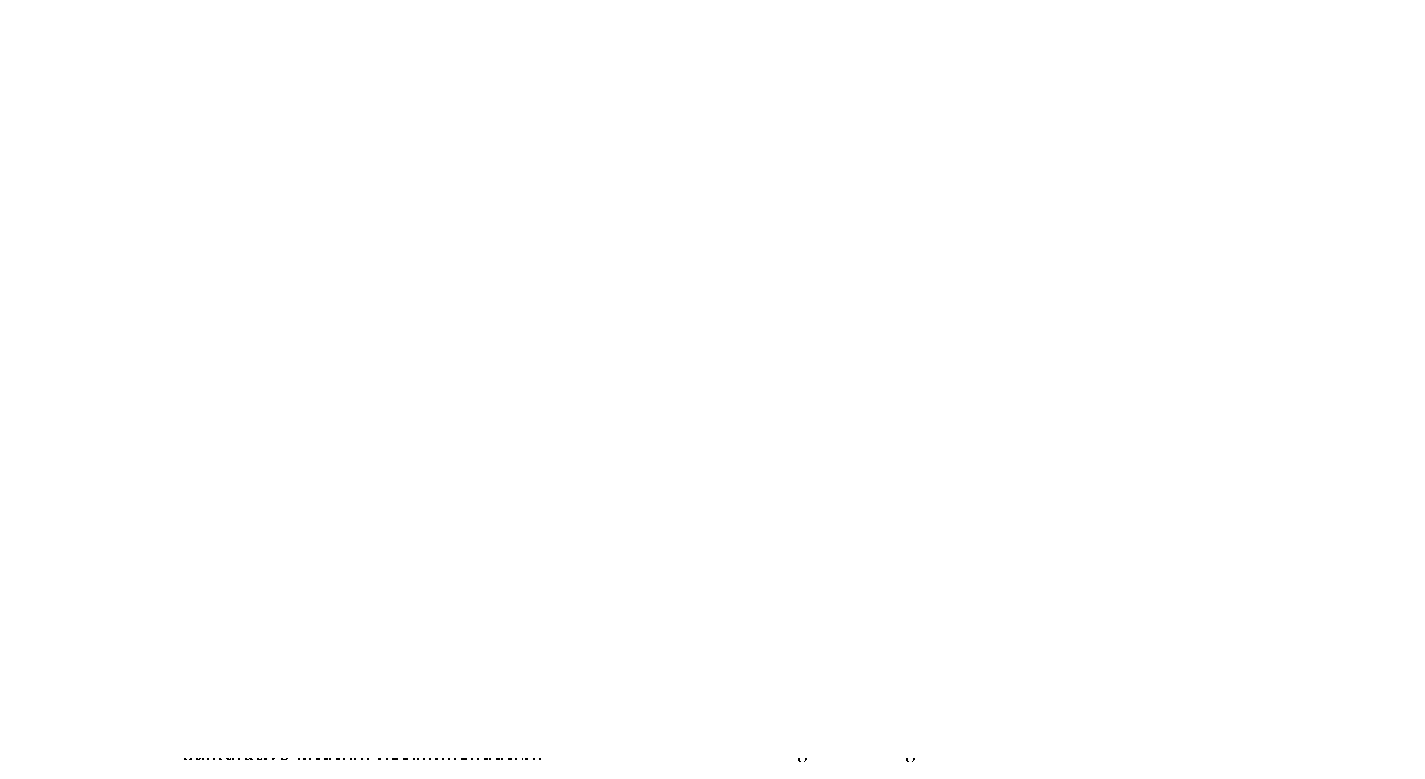
\includegraphics[width=4.5in]{./images/system.eps}
%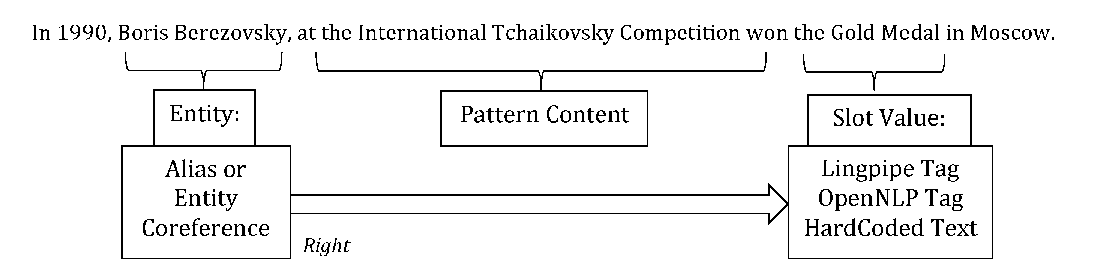
\includegraphics[width=6in]{./images/Pattern.eps}
%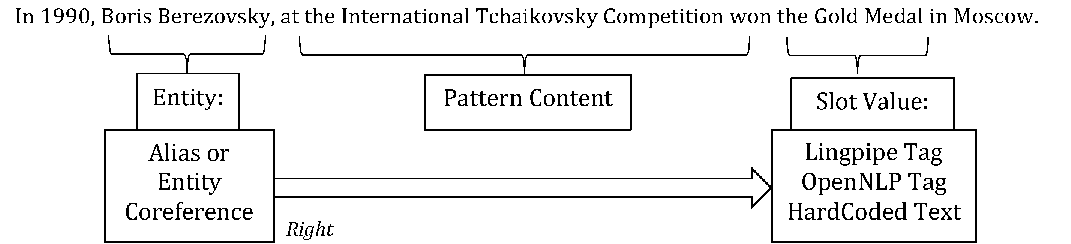
\includegraphics[width=6in]{./images/Pattern-eps-converted-to.pdf}
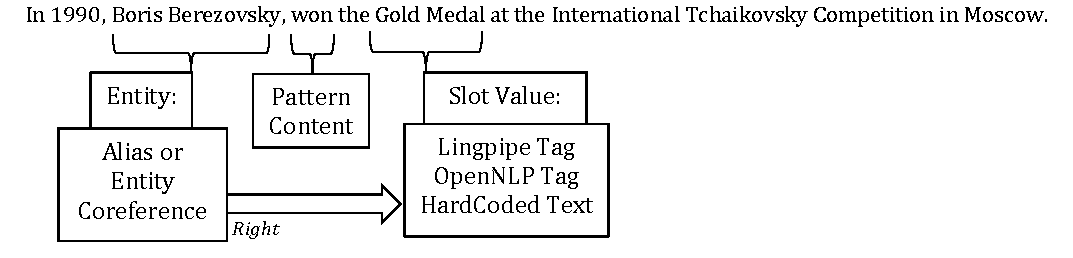
\includegraphics[width = 13cm]{./images/Pattern-crop.pdf}
% cropped pdf created using $ pdfcrop Pattern.pdf
\vspace*{-.1in} \caption{Pattern Matching with Slot Value on the Right Side of Entity. }\label{fig:pattern}
\vspace*{-.2in}
\end{figure}

In the data set, we are given a date range of documents as training data. Instead of building a classifier we use pattern matching methods to find corresponding slot values for entities. 
Pattern matching is simple to manipulate results and implement. Additionally, a classifier approach is more difficult to evaluate and explain results due to the lack of proper training data.

With the documents indexes generated by the Wikipedia Citation, we first fetch the sentences containing entites by using alias names and coreference information provided by Lingpipe tags\footnote{http://alias-i.com/lingpipe/}. Then use these senteces to match patterns and when patterns matched, generate SSF results.

\begin{algorithm}
  \caption{Slot Value Extraction Pseudocode}
  \textbf{List of entities $\mathcal{E} = \{e_0, \ldots, e_{170}\}$}\\
  \textbf{List of patterns $P = \{p_0, \ldots, p_{|P|}\}$}\\
  \textbf{List of streamitems containing entities $\mathcal{S} = \{s_0, \ldots, s_{|\mathcal{S}|}\}$}\\
  
  \begin{algorithmic}%[1]
    \FOR{$si \in \mathcal{S}$}
      \FOR{$sentence \in si$}
        \FOR{$entity \in \mathcal{E}$}
	  \IF{Contains($sentence$, $entity$)}
          %%\IF{check\_pattern(sentence, pattern)}
            \FOR{$pattern \in P $ suitable for $entity$} 
              \IF{Satisfies($sentence$, $pattern$)}
                \STATE Emit($sentence$, $pattern$)
              \ENDIF
	    \ENDFOR
          \ENDIF
        \ENDFOR
      \ENDFOR
    \ENDFOR
  \end{algorithmic}
\end{algorithm}


\subsubsection{Rule Engine}

\textbf{Format of Patterns.} A pattern is defined as a record representing knowledge going to be added to a KB. A pattern $\mathcal{P}$ is represented as a five-tuple $\mathcal{P} = \langle p_1, p_2, p_3, p_4, p_5 \rangle$.


The first value, $p_1$ represents the type of entity. These entity types are in the set $\{ \text{\tt FAC}, \text{\tt ORG}, \text{\tt PER} \}$ where \texttt{FAC} represents a type of facility, \texttt{ORG} represents an organization and \texttt{PER} represents a person. \texttt{FAC}, \texttt{ORG} and \texttt{PER} are Lingpipe entity types. The $p_2$ represents a slot name. A list of slot names is present in Table~\ref{table:slotNameOntology}. The third element $p_3$ is the pattern content. This is a string found in the sentence. The extractor looks for this exact string or pattern in a sentence. The pattern evaluator uses a direction (\texttt{left} or \texttt{right}) found in $p_4$ to explore sentence. The final element $p_5$ represent the slot value of a pattern. This %When we match one pattern, we match all the 
%fields except the third field, which is extracted as the final result.
The type of slot value may be the entity type tagged by Lingpipe, a noun phrase (\texttt{NP}) tagged by OpenNLP or a hard-coded phrase. For these three kinds of patterns, we implement them in different 
ways accordingly. Next, we explain the patterns with more details, an example can be found in Figure~\ref{fig:pattern}. 

\textbf{Types of patterns}
There are three types of patterns distinguished by different types of slot values in the patterns. The matching methods using these three types of patterns are implememented according to the different information and structures of slot values.

 
\textbf{Type I.} This pattern type is driven by the slot value type, a pattern tagged by Lingpipe. For example, pattern $\langle$\texttt{PER, FounderOf, \textit{founder}, right, ORG}$\rangle$. \texttt{PER} means 
that the entity we are finding slot values for a PER entity; \texttt{FounderOf} means this is a pattern for FounderOf slot. \textit{founder} is the anchor word we are match in a sentence; \texttt{right} means that we are going to the right part of the sentence to match the pattern and find the slot value; ORG means the slot value should be a ORG entity.

\textbf{Type II.} This pattern type is unique because it only looks for a slot value tagged as noun phrase (NP) by OpenNLP.\@ For example, pattern $\langle$\texttt{PER, AwardsWon, \textit{awarded}, right, NP}$\rangle$. This pattern can be interpreted as that we are looking for a noun phrase after the \textit{awarded} since that noun phrase may represent an award. Titles and awards are usually not the Lingpipe entities, hence the use of the OpenNLP noun phrase chunker to fetch the noun phrases.

\textbf{Type III.} Some relations are best discovered by hard coding the slot values. Examples of these include time phrases: $\langle$\texttt{PER, DateOfDeath, \textit{died}, right, \textit{last night}}$\rangle$. In this pattern, \textit{last night} means we are looking for exactly the phrase \textit{last night} to the right of \textit{died}. This pattern is inspired by the intuition that in news articles, people often mention that somebody died last night instead of mentioning the accurate date information and Lingpipe tends not to tag phrases like \textit{last night} as a DATE entity. 


\subsubsection{Constraints - Inference}

The SSF output of streaming slot value extraction is noisy. The data contains duplicates and incorrect extractions. We can define rules to sanitize the output only using the information present at this stage. The input file is processed in time order, in a tuple-at-a-time fashion to minimize the impact on accuracy. We define two classes of rules: \textit{deduplication} and \textit{inference} rules.

The output contains many duplicate entries. As we read the list of extracted slots we create rules to define ``duplicate''. Duplicates can be present in a window of rows; we use a window size of 2 meaning we only be adjacent rows. Two rows are duplicates if they have the same exact extraction, or if the rows have the same slot name and a similar slot value or if the extracted sentence for a particular slot types come from the same sentence.

 New slots can be deduced from existing slots by defining inference rules. For example, two slots for the task are ``FounderOf'' and ``FoundedBy''. A safe assumption is these slot names are biconditional logical connectives with the entities and slot values. Therefore, we can express a rule ``X FounderOf Y'' equals ``Y FoundedBy X'' where X and Y are single unique entities. Additionally, we found that the slot names ``Contact\_Meet\_PlaceTime'' could be inferred as ``Contact\_Meet\_Entity'' if the Entity was a FAC and the extracted sentence contained an additional ORG/FAC tag. We also remove erronious slots that have extractions that are several pages in length or tool small. Errors of extracting long sentences can typically be 
attributed to poor sentence parsing of web documents. We have some valid ``small'' extractions. For example a comma may separate a name and a title (e.g. ``John, Professor at MIT''). But such extraction rules can be particularly noisy, so we check to see if the extracted values have good entity values.





\subsubsection{A short discussion}

